Augmentations is a powerful regularization technique that helps the netwrk to generalize better [cite Wang 2017] and is an effective solution for a situation with the lack of labeled data [cite Yang 2022]. The main idea behind the augmentation is to increase the diversity of training data, when the acquisition of the real training data is expensive. Augmenting existing images creates the new synthetic samples which are hypotetically very close to the original true distribution of images. However one should be very cautios regarding the type of augmentations that can be used. Augmentation must enrich the dataset, however should not change the semantics hidden in each image. The peculiarity of current research is the pair-wise correspondense between the DIC input and the output fluorescence. One should not change the input in such a way that the fluorescence signal could not be infered from it. Therefore the following augmentations have been used on cropped images:

\begin{itemize}
	\item \textbf{Flipping}: Flip the crop horizontally (30\% chance), vertically (30\% chance) or both.
	\item \textbf{Random rotation}: Rotates the crop by a random angle.
	\item \textbf{Random scaling}: Reduces crop size by 100 (20\% chance), 50 (20\% chance) or 20 (60\% chance) pixels from each side (down, top, left, right).
	\item \textbf{Contrast}: Descreases an image constrast in twice (50\% chance), or triples it (50\% chance). Applied with 20\% chance.
	\item \textbf{Defocus blur}: Imitates a defocus blur of severity level 4 (see section [TODO cite section]) on an image with 20 \% chance.
\end{itemize}

\paragraph{Special augmentations for rotation and scaling}

Augmentations are chosed to be applied during training and the reason for that is to preserve the same conditions regarding the size of the datasets in order to have a fair comparison between approaches. For example, one decides to augment 20\% of images and add them to an original dataset in order to expand it. Then the comparison between training with and without augmentations would be unfair as the sizes of the datasets are different, and it is not clear wether the performance improvement or decrease comes from the longer training (enlarged dataset) or augmentations. 

Since augmentations are applied on crops directly during training there is a possibility to improve the rotation and scale of crops. The problem with this augmentations are depicted in the Figure \ref{fig:smart-augments} - after applying them there will appear a gray background, that wuold be filled with zeros in PyTorch implementation. However in since one has an original image where the crop has been cut out, one can easily restore background with original values and escape this problem alltogether.

\begin{figure}[H]
	\begin{center}
		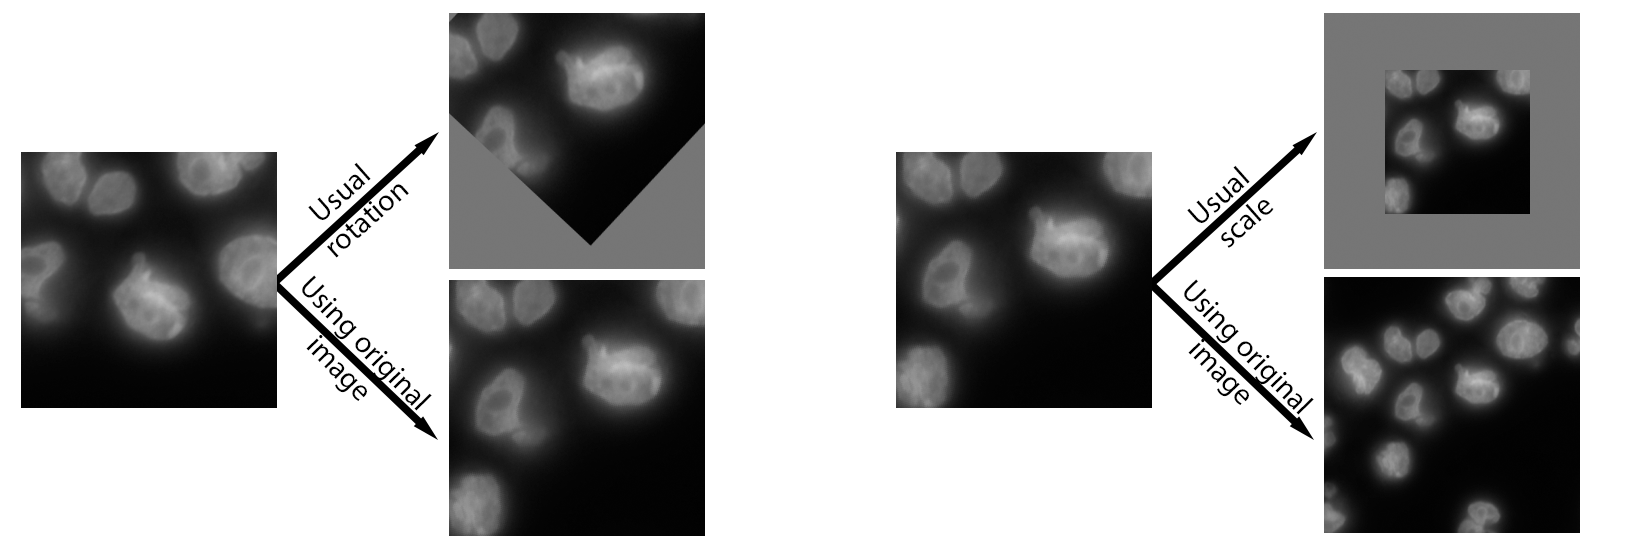
\includegraphics[width=0.7\linewidth]{bilder/model training/smart augmentations.png}
		\caption{Using original image for rotation and scaling augmentations}\label{fig:smart-augments}
	\end{center}
\end{figure}

Applying augmentations in combination with other regularization techniques has proven to be helpful against overfitting for the nuclei and ER training. Therefore it is recommened to use it in further research as well.